\chapter{The Software Project Architecture}
\label{chap:arch}

The software package was designed and developed with extensibility in mind.
It allows easily adding new features, specifying different subsets of data and converting them into various format without breaking older experiments.
Classifiers and preprocessing methods are implemented as children of abstract classes to allow users to add new algorithms.
The entire experiment is configured in a special configuration file.
It precisely defines conducted experiments and the evaluation metrics.

A new folder for statistics is created every run to prevent accidental overwriting of already obtained results.
The entire project runs in Python of version at least 3.6\footnote{\url{https://python.org}} and bash\footnote{\url{https://gnu.org/software/bash}}.
Various libraries are utilized for both higher performance and easier maintainability.
All classes and files have documentation strings which should be sufficient for detailed understanding.
In this chapter, we only describe the high-level overview.

\autoref{tab:files} displays definitions of special files used for controlling the run of the software project.
Their exact usage is explained in appropriate sections.

\begin{table}[h]

\centering
\begin{tabular}{ll}
\toprule
\textbf{name of file}& \textbf{purpose} \\
\midrule
instance file		 & stores preprocessed instances \\
intermediate file	 & used for generating Geneea file \\
Geneea file			 & contains extra linguistics data for instances \\
experiments file	 & configures the experiments conducted \\
\bottomrule
\end{tabular}

\caption{File definition}\label{tab:files}
\end{table}

\todoA{add libraries used - as another appendix??}


\section{Experiments File}

This YAML\footnote{\url{https://yaml.org}}  file contains entire configuration of experiments conducted.
It lists classification tasks and defines evaluation.
Each task is a definition of a classifier.
Evaluation element is a definition what properties should be plotted in a graph.

Experiments file has the following format.
The root element is a dictionary with three parts;
\texttt{config}, \texttt{tasks} and \texttt{graphs}.
An example file can be found bellow.

\begin{code}
config:
  chunks: 10
tasks:
  - name: 'zero-R'
    classificator: 'baseline'
    features:
      - REVIEWLEN
      - UNIGRAMS
    preprocessing:
      - 'mutualinformation'
      - 'featurematrixconversion'
    extra_data: []
    config:
      algorithm: 'zero-R'
      features_to_select: 2
graphs:
  - name: 'baseline'
    data:
      zero-R:
        - 'f-measure'
\end{code}

The config section is another dictionary.
It has only one element -- \texttt{chunks}.
It specifies the argument~$k$~for k-fold cross-validation.

The section \texttt{experiments} is a list of classification tasks.
Each element is a dictionary specifying the exact parameters.
Descriptions of individual fields is in \autoref{tab:exp_dict}.
The list \texttt{features} consists of names as defined in FeatureSetEnum.
The exact definition can be found in \autoref{tab:fea_grp}.
\texttt{extra\_data} is any property of instances available in the raw data.
An example is the original text or business attributes.

\begin{table}[h]

\centering
\begin{tabular}{lll}
\toprule
\textbf{element name} & \textbf{type} & \textbf{meaning}\\
\midrule
name 			& string	& identification referred to in graphs\\
classificator 	& string	& used classifier\\
features 		& list		& used features \\
preprocessing 	& list		& applied preprocessors in order\\
extra\_data 	& list 		& extra attributes passed to the first preprocessor \\
config			& dict		& extra configuration for all parts of pipeline \\
\bottomrule
\end{tabular}

\caption{Experiment Configuration}\label{tab:exp_dict}
\end{table}


The last section \texttt{graphs} is used for specifying what graphs will be plotted.
It is a list of individual figures.
Each figure is a dictionary of two elements; \texttt{name} and \texttt{data}.
Name specifies the filenames of the resulting graph ---
for each figure png and csv files will be created.
Element \texttt{data} specifies what evaluation metrics for what classifiers will be used.
It is a dictionary of experiment names, values being a list of all metrics to be output.

\section{Parts Overview}

The project is divided into three main parts as shown in \autoref{fig:arch_process}.
These parts are executed with make\footnote{url{https://www.gnu.org/software/make}} with dependencies properly set.
The entire project can be therefore run simply by \texttt{make run}.
We describe each part in a separate subsection.

\begin{figure}[h]
    \centering
	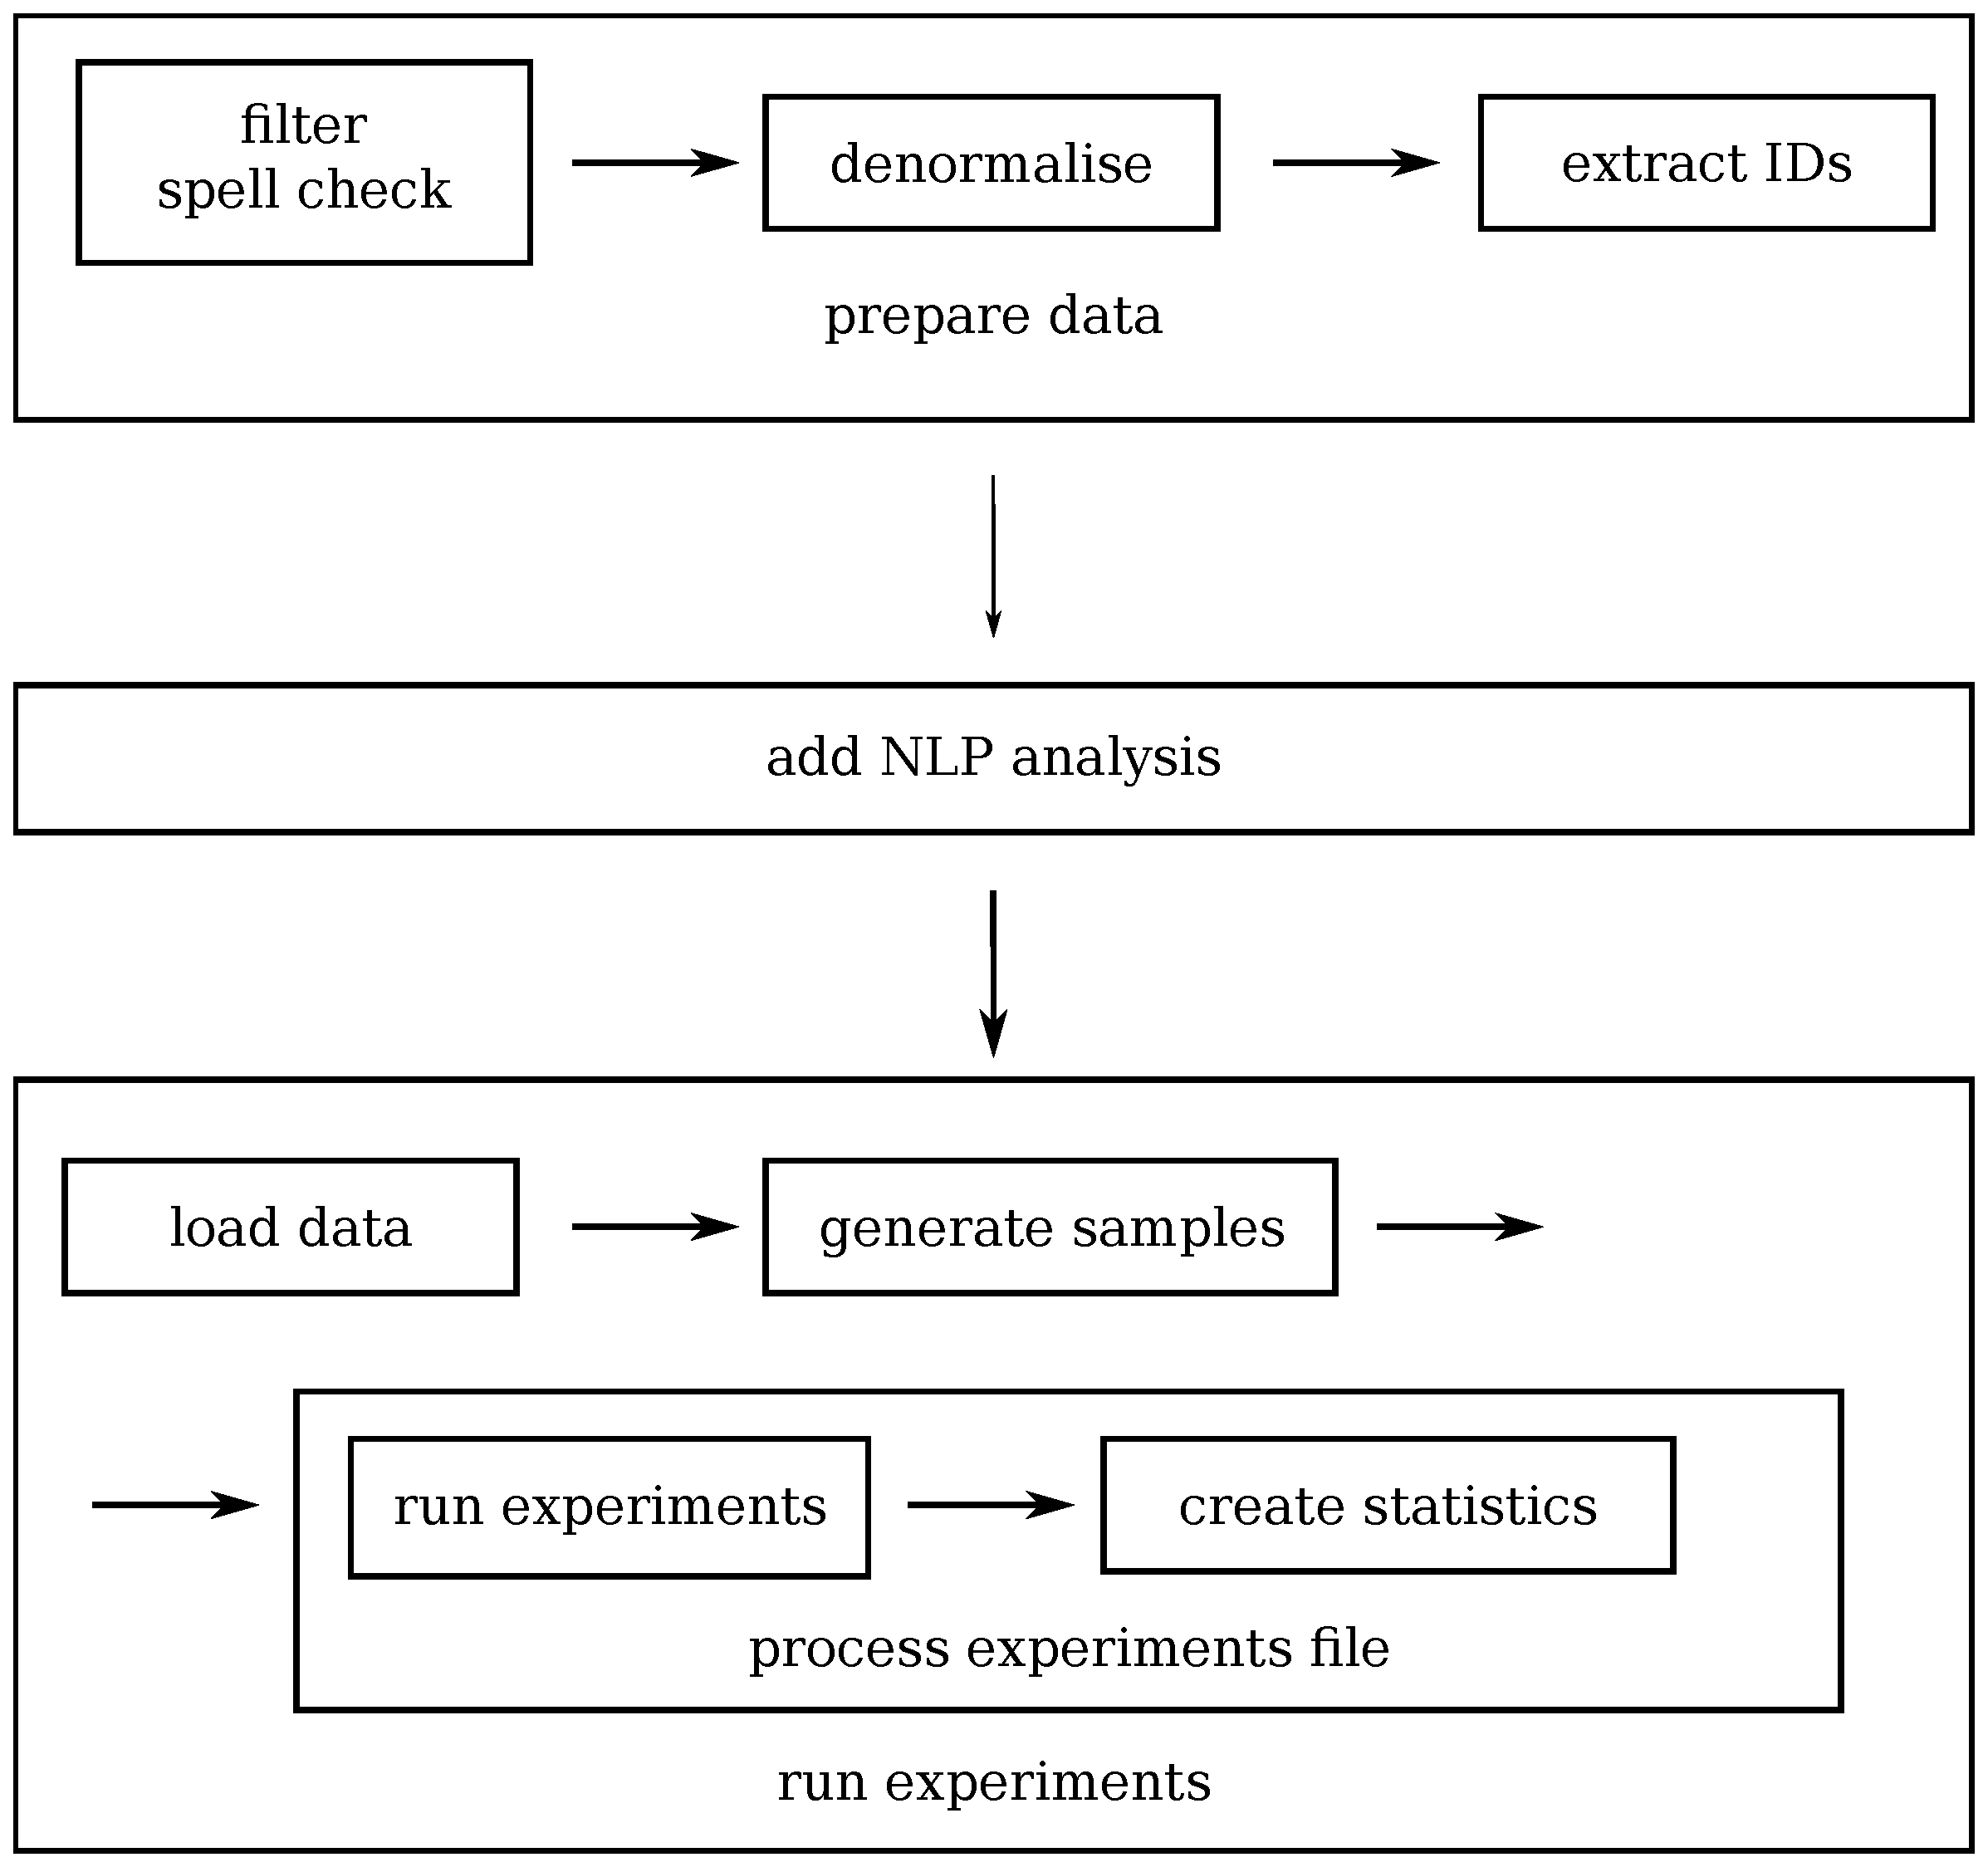
\includegraphics[width=10cm]{figures/arch_process.eps}
	\caption{Architecture Design}\label{fig:arch_process}
\end{figure}


\subsection{Data Preparation} 

This part itself can be run by:

\begin{code}
make data/data.json
\end{code}

All scripts for preparing data are in the folder \texttt{denormalization}.
These scripts prepare the instance and intermediate files.
Preparation is executed by:

\begin{code}
./denormalization/denormalize.sh ../data/dataset data/data.json data/ids
\end{code}

The first argument is a directory with extracted archive of the Yelp Dataset.
The second argument is a path to the instance file and the last one to the intermediate file.
The script itself filters out not-needed reviews.
Also, it adds the information from the spell checker.
Subsequently, it joins reviews and business by replacing business id by the actual data.
The result is written in the instance file.
Finally, it prepares list of all IDs of used reviews into the intermediate file one ID per line.
The exact description of data and files format can be found in \autoref{app:a}.



\subsection{Geneea Analysis}

The Geneea analysis takes the text of the reviews and computes some additional linguistics data.
It is done on a separate server for performance reasons.
The geneea file is created and transferred to the local computer.
Because of this, make only notifies users when it is needed to supply a new version of the geneea file.
The resulting file must be named \texttt{data/geneea.json}.



\subsection{Running Experiments}

Experiments are handled by \texttt{process\_data.py} and can be run with:

\begin{code}
make run
\end{code}


\subsubsection{Load Data}

Class \texttt{Data} is created by \texttt{process\_data.py}.
It is defined in file \texttt{load\_data.py} and is used for loading data.
It stores raw data in Pandas DataFrame to achieve easier manipulation without compromising performance.

\texttt{process\_data.py} uses this class for generating samples and getting the right data.
Whenever a new sample is generated, the raw data is filtered out and split into chunks.
The chunks are stored in an instance of \texttt{Sample}.
\texttt{Sample} still keeps only raw data.
Anytime a dataset is accessed all features are regenerated to ensure everything is up-to-date.


\subsubsection{Conduct Experiments}

Once all data is loaded in the memory, experiments are conducted.
The file \texttt{process\_data.py} reads the experiments file, create instances of classifiers and preprocessors.
These instances are then fed with data from the instance of \texttt{Sample}.
All tasks are guaranteed to be run on the exactly same data to ensure comparability of results.

Both training and testing is implemented by a pipeline.
The units of the pipeline are preprocessors and a classifier.
The preprocessors are in the same order as in the experiment file.
A preprocessor must be defined in the directory \texttt{preprocessors} and be a child of \texttt{preprocessors/preprocessingbase.py}.
Also, its name must be added into \texttt{preprocessors/\_\_init\_\_.py}.

Since the input and output formats of the pipeline units are arbitrary,
it is up to the user to ensure compatibility of adjacent units.
This holds except for the input of the first preprocessor and the output of the classifier.
The first preprocessor in the pipeline must take feature\_dict with possibly additional data specified in \texttt{extra\_data} as returned by \texttt{load\_data.Data.get\_feature\_dict}.
The classifier must return the predicted label.
The output of training is not stored.
Note that for most classifiers, it is needed to run conversion to matrix as a last preprocessor (\texttt{featurematrixconversion.py}).

The pipeline is the same for both training and testing data with the guarantee that
training data is always passed first and classifier is called train and classify for
training and testing data, respectively.

When all tasks are performed, results are output.
All helpers classes for writing statistics are defined in \texttt{statistics.py}.
For storing evaluation data, class \texttt{DataGraph} is used.
It servers as a buffer for evaluation data and provides API for data manipulation.
An instance of this class is passed to \texttt{Statistics},
which handles the actual data plotting and writing to files.
